\subsection{Un module type : le référentiel des langues}
\label{section:eyrolles_ref-langues}

Le référentiel des langues est l'un des nombreux référentiels administrables de l'application décrits dans la partie~***.

Il est implémenté sous la forme d'un module nommé \texttt{ey\-Referential\-Language} qui utilise \asladmin. En effet, le module doit offrir les fonctionnalités suivantes, qui sont offertes par défaut par le \aplugin\ :
\begin{itemize}
	\item le listings des langues contenues dans la base de données ;
	\item l'ajout et la modification d'une langue ;
	\item la suppression d'une langue.
\end{itemize}

Le module des langues a été choisi pour être décrit car il peut être considéré comme un module qui, tout en restant très simple, est typique de l'application. Les paragraphes suivants rentrent dans le détail de son implémentation, et l'annexe~\ref{section:annexe_eyrolles_ref-langues} regroupe son code et des captures d'écran.


\subsubsection{Arborescence}

L'arborescence de \texttt{eyReferentialLanguage} suit les règles classiques d'organisation d'un module \asf\ et intègre les fichiers nécessaires au bon fonctionnement de \asladmin\ :

\begin{verbatim}
eyReferentialLanguage/
  actions/
    actions.class.php
  lib/
    config/
      slAdminConfigurationEyReferentialLanguage.class
  templates/
    _form.php
    _listTableRow.php
    listSuccess.php
    newSuccess.php
\end{verbatim}

L'organisation des fichiers de \atemplate\ ne suit pas exactement les consignes énoncées en partie~\ref{section:eyrolles_sladmin_view}. En effet, dans la classe de configuration, on a préféré utiliser le nom de \apartial\ \texttt{listTableRow} au lieu de \texttt{list\_row}. Par ailleurs, le \apartial\ \texttt{form} est appelé dans le \atemplate\ \texttt{new}.


\subsubsection{Schéma de la base de données}

Le données du référentiel des langues sont stockées dans une seule table de la base de données nommée \texttt{EyReferentialLanguage}. Elle contient les champs suivants : \texttt{id}, \texttt{label}, \texttt{description} et \texttt{created\_by}. Le champ \texttt{id} est la clé primaire de la table, qui sert à identifier de façon unique chaque langue. Quant au champ \texttt{created\_by}, il est utilisé en tant que clé étrangère vers la table des utilisateurs de l'\aintranet\ \texttt{sfGuardUser} : cette liaison permet de retrouver le créateur de la langue.

Le schéma permettant de créer cette table dans la base de données est repris dans le listing~\ref{listing:eyrolles_ref-langues_schema}. Pour expliciter ce format, un diagramme \auml\ équivalent est proposé en figure~\ref{figure:eyrolles_ref-langues_uml}.

\begin{figure}
	\centering
	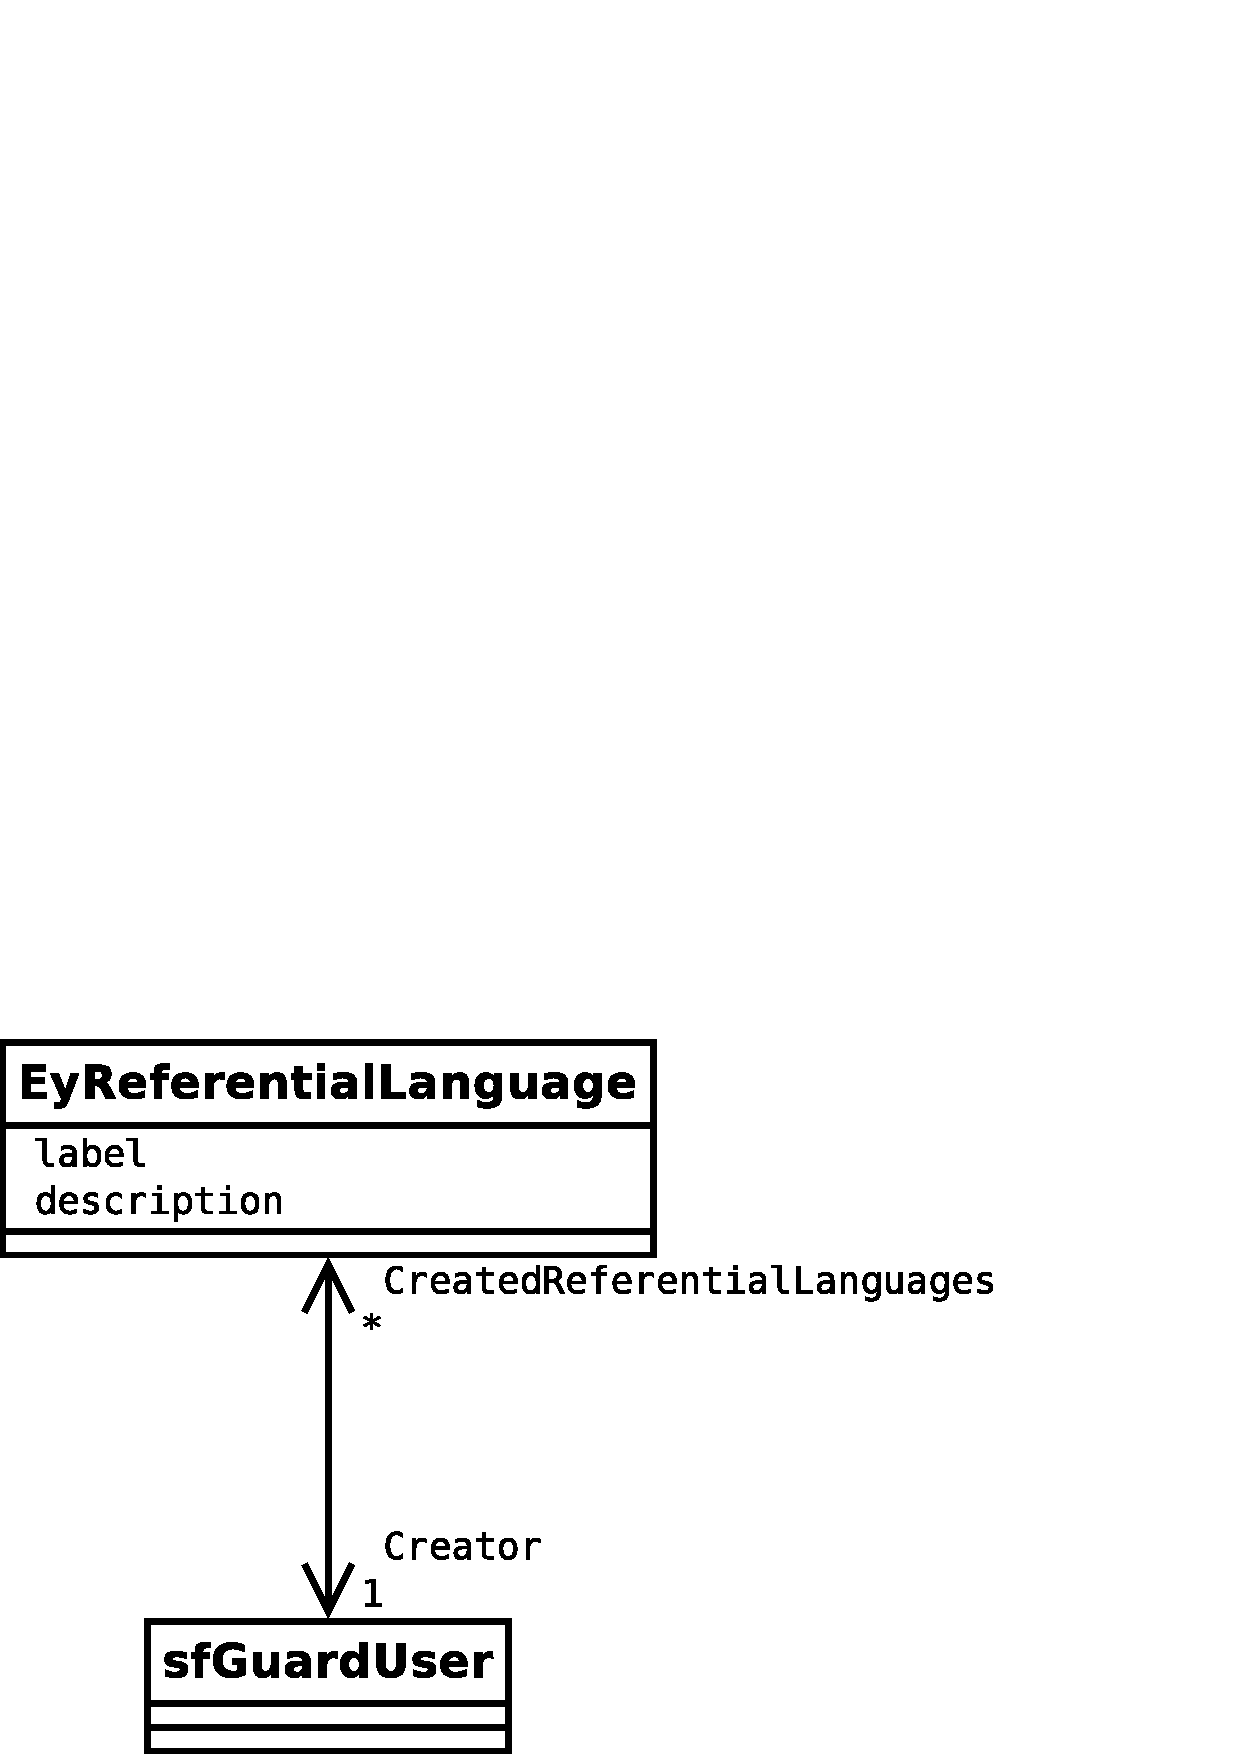
\includegraphics[scale=0.4]{eyrolles_ref-langues_uml}
	\caption{Représentaion \auml\ de la table du référentiel des langues}
	\label{figure:eyrolles_ref-langues_uml}
\end{figure}

On peut noter l'utilisation des mots-clés \texttt{Timestampable} et \texttt{SoftDelete} listés dans la partie \texttt{actAs}. Ce sont ce que l'on appelle des \emph{behaviors} \adoctrine\ : ils peuvent être assimilés à des comportements personnalisés que l'on veut donner à une table.

En effet, le \abehavior\ \texttt{Timestampable} ajoute automatiquement deux champs \texttt{created\_at} et \texttt{updated\_at} dans la table. Respectivement, ils sont remplis automatiquement par une date quand un enregistrement est crée et quand il est mis à jour. En plus de garder une trace du créateur de la langue, \texttt{Timestampable} conservera alors les données temporelles de modification de la table.

Le \abehavior\ \texttt{SoftDelete}, quant à lui, permet de ne jamais supprimer un enregistrement de la base de données. En fait, il ajoute un champ \texttt{deleted\_at} : quand on demande la suppression d'un enregistrement, sa valeur est affectée à la date de la pseudo délétion, sinon sa valeur est nulle. Les différentes requêtes \adoctrine\ écrites par le développeur sont alors automatiquement modifiées pour ignorer les enregistrements qui sont sensés avoir été supprimés. Dans le cas d'\aey, \texttt{SoftDelete} permet d'implémenter nativement l'archivage des données au cas où le client aurait besoin de les restaurer ou d'en générer des statistiques.


\subsubsection{Configuration}

La classe de configuration nécessaire pour \asladmin\ est accessible dans le listing~\ref{listing:eyrolles_ref-langues_config}.

Sans expliciter de façon fastidieuse toutes les options utilisées, elle définit globalement les paramètres suivants :

\begin{itemize}
	\item la classe de modèle à utiliser ;
	\item la requête à utiliser pour récupérer les langues à afficher sur la page de listing (listing~\ref{listing:eyrolles_ref-langues_table}) ;
	\item le champ sur lequel les langues seront triés ;
	\item le nombre maximum de langues affichées sur la page de listing ;
	\item le titre des colonnes du tableau de la page de listing ;
	\item le \apartial\ à utiliser pour afficher une ligne du tableau de listing ;
	\item les classes de formulaire à utiliser.
\end{itemize}


\subsubsection{Routes}

Le fichier de \arouting\ du module est accessible dans le listing~\ref{listing:eyrolles_ref-langues_routing}.

\texttt{eyReferentialLanguage\_batch} est une route classique. La valeur du champ \texttt{url} correspond à l'adresse que l'utilisateur va entrer dans son navigateur pour accéder à l'action \texttt{batch} du module \texttt{eyReferentialLanguage}. L'option \texttt{sf\_method} indique quelle méthode \ahttp\footnote{Dans le protocole \ahttp, une méthode est une commande spécifiant un type de requête, c'est-à-dire qu'elle demande au serveur d'effectuer une action. \cite{http}} l'utilisateur doit appeler pour que la route soit accessible. Dans le cas de cette route, la méthode est \texttt{POST}, ce qui correspond en fait à la validation d'un formulaire.

La route \texttt{eyReferentialLanguage}, quant à elle, utilise la classe de \arouting\ avancée \texttt{sfDoctrineRouteCollection}. Cette classe intégrée au \afm\ \asf\ a la particularité de générer tout un ensemble routes qui correspondent à des actions de bases. Par exemple, des actions générées sont \texttt{ey\-Re\-fe\-ren\-tial\-Lan\-guage\_\-list}, \texttt{ey\-Re\-fe\-ren\-tial\-Lan\-guage\_\-new}, \texttt{ey\-Re\-fe\-ren\-tial\-Lan\-guage\_\-edit}, correspondent respectivement aux actions \texttt{list}, \texttt{new}, \texttt{edit}, et redirigent respectivement vers le listing des langues, la création d'une langue et son édition.


\subsubsection{Actions}

Les actions du module, situées dans la classe \texttt{ey\-Referential\-Language\-Actions}, reposent sur les actions de base d'\aey\footnote{Voir le listing~\ref{listing:eyrolles_base_actions}}, qui reposent elles-mêmes sur les actions de \asladmin. Elles sont accessibles dans le listing~\ref{listing:eyrolles_ref-langues_actions}.

On remarque que seule l'action \texttt{edit} est redéfinie. En effet, on y ajoute le nom de la langue que l'on est en train d'éditer dans le fil d'Arianne\footnote{Sur un site web, un fil d'Ariane représente l'arborescence des rubriques que le visiteur a traversées depuis la page d'accueil.\cite{breadcrumb}\\Exemple : \texttt{Accueil > Référentiels > Langues > Liste}}. Toutes les autres actions comme \texttt{list} ou \texttt{new} sont en réalité déjà écrites dans les actions de base de \asladmin. Le fait qu'il y ait au final peu de code à écrire est un bon signe : c'est un gain de temps pour le développeur et c'est une bonne opportunité pour ne pas intégrer de \abug. C'est justement ce genre d'avantage qui a incité à utiliser \asladmin\ dans \aey.

Dans les actions de base \texttt{eyBaseAdminActions}, la méthode \texttt{init\-Bread\-crumb()}, qui initialise le fil d'Arianne, est appelée dans la méthode \texttt{pre\-Execute()} : ainsi, le fil d'Arianne est initialisé dans chaque action de l'application \aey. La méthode \texttt{initBreadcrumb()} est surchargée dans \texttt{ey\-Referential\-Language\-Actions} : au mot \textit{Accueil} présent sur toute les pages, on ajoute \textit{Référentiels} puis \textit{Langues}. C'est un bon exemple de la façon typique de surcharger les classes de \asladmin.

Le module du référentiel des langues restant un module très simple, les actions de \asladmin\ n'ont pas trop eu a être surchargées. Dans d'autres modules, qui intègrent une logique métier plus poussée, il est nécessaire d'apporter une surcharge plus importante et d'écrire des actions supplémentaires spécifiques.


\subsubsection{Affichage de la vue}

Les vues, contrairement aux actions, n'ont pas déjà été écrites dans \asladmin\ : c'est au développeur de les implémenter en totalité.

Les \atemplates\ et les \apartials\ utilisés dans le module sont les suivants :

\begin{description}
	\item[\texttt{listSuccess.php}] \atemplate\ du listing des langues (listing~\ref{listing:eyrolles_ref-langues_template-list})
	\item[\texttt{\_listTableRow.php}] \apartial\ des lignes du tableau de listing (listing~\ref{listing:eyrolles_ref-langues_template-row})
	\item[\texttt{newSuccess.php}] \atemplate\ de création d'une langue (listing~\ref{listing:eyrolles_ref-langues_template-new})
	\item[\texttt{\_form.php}] \apartial\ du formulaire de création (listing~\ref{listing:eyrolles_ref-langues_template-form})
\end{description}

Étant donné la quantité de concepts à acquérir pour comprendre les subtilités de la vue, le fonctionnement de ces fichiers de \atemplate\ ne sera pas décrit ici en détail. Pour en savoir plus, il est toutefois possible de se référer à la documentation du \afm\ \asf\cite{thebook}.

Voilà tout de même quelques clés :

\begin{itemize}
	\item les fonctions \texttt{url\_for()} et \texttt{link\_to()} permettent de générer des liens hypertexte à partir des routes passées en paramètre ;
	\item la fonction \texttt{image\_tag()} permet de générer la balise d'une image donnée pour l'afficher dans le navigateur ;
	\item dans \texttt{\_listTableRow.php}, la variable \texttt{\$subject} représente l'instance de l'objet de langue à afficher sur la ligne du tableau ;
	\item la fonction \texttt{include\_partial()} permet d'inclure un \apartial\ dans un \atemplate\ : c'est de cette manière que \texttt{\_form.php} est inclus dans \texttt{new\-Success.php} ;
	\item l'inclusion de \texttt{\_listTableRow.php} dans \texttt{listSuccess.php} se fait dans le \awidget\ du tableau \texttt{\$widgetTable}, qui provient de \asladmin ;
	\item le rendu HTML du formulaire est ici généré automatiquement par \asf\ (en se basant sur le schéma de la base de données) en utilisant l'instruction \texttt{echo \$form}.
\end{itemize}
